
%This is the segment that can be as long or short as needed to finish in time. Leave to end.
%Performance Analysis. Discuss impact of number of planes, size of planes, etc, with collected data. Highlight areas of improvement, engineering challenges with memory usage, reuse of buffers, reduction of memory usage by parameter tweaking, stream overlapping. Try to benchmark against other algorithms if have time, but probably won't.
\chapter{Performance Analysis}
\label{chap:analysis}


\begin{figure}[ht]
    \centering
    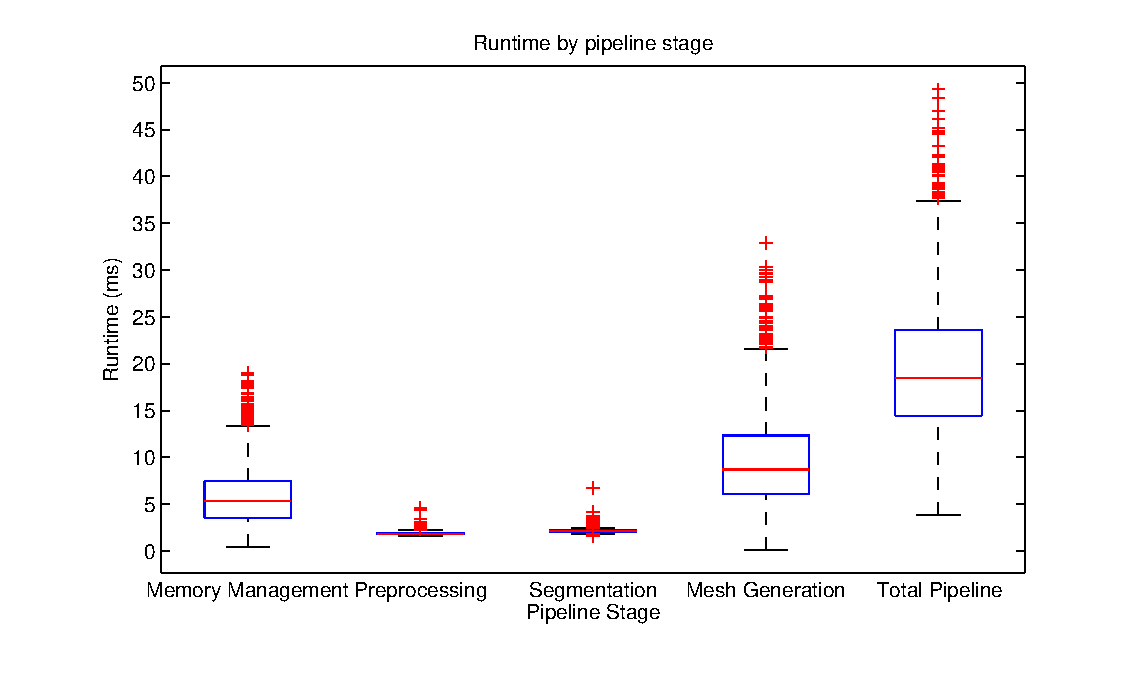
\includegraphics[width=1.0\textwidth]{RuntimeByPipelineStage.eps}
    \caption{Pipeline runtime broken down by stage.}
    \label{fig:runtimebystage}
\end{figure}

\begin{figure}[ht]
    \centering
    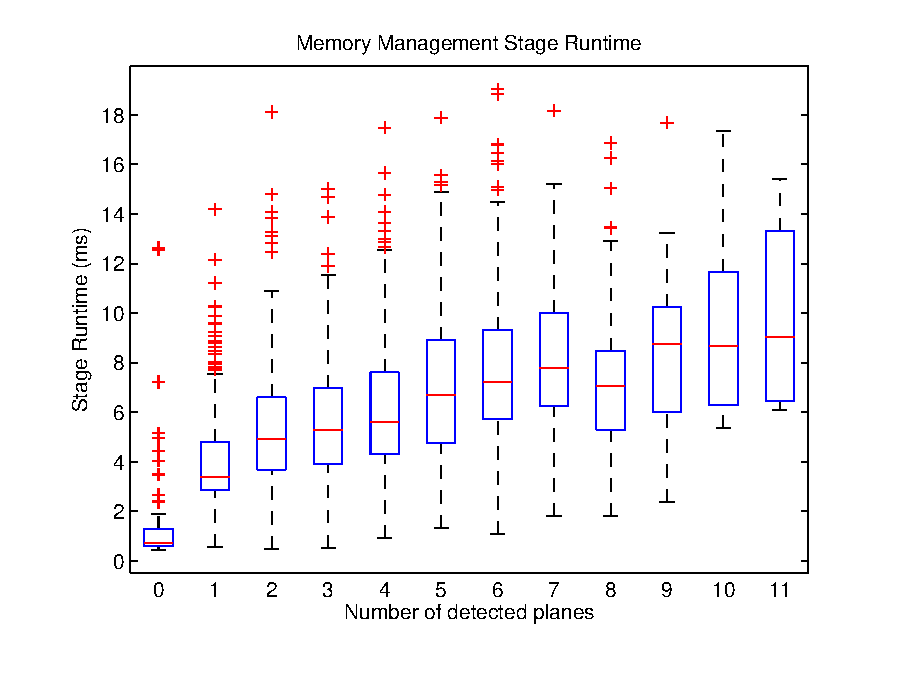
\includegraphics[width=0.7\textwidth]{MemoryManagementByNumPlanes.eps}
    \caption{Runtime of the memory management stage by number of detected planes.}
    \label{fig:memorymangementplanes}
\end{figure}


\begin{figure}[ht]
    \centering
    \includegraphics[width=0.7\textwidth]{PreprocessingByNumPlanes.eps}
    \caption{Runtime of the preprocessing stage by number of detected planes.}
    \label{fig:preprocessingplanes}
\end{figure}



\begin{figure}[ht]
    \centering
    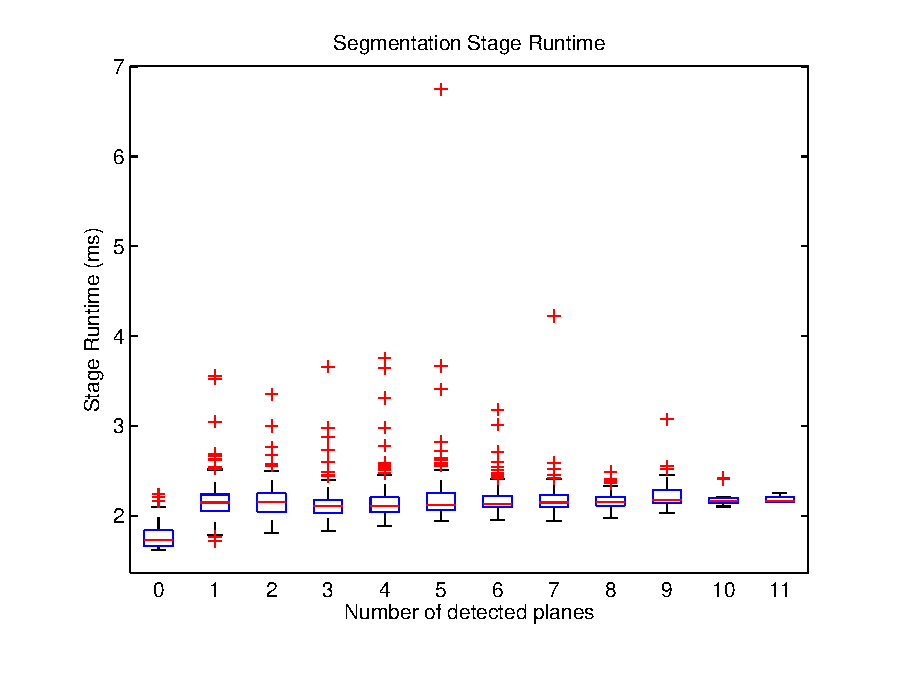
\includegraphics[width=0.7\textwidth]{SegmentationByNumPlanes.eps}
    \caption{Runtime of the segmentation stage by number of detected planes.}
    \label{fig:segementationplanes}
\end{figure}



\begin{figure}[ht]
    \centering
    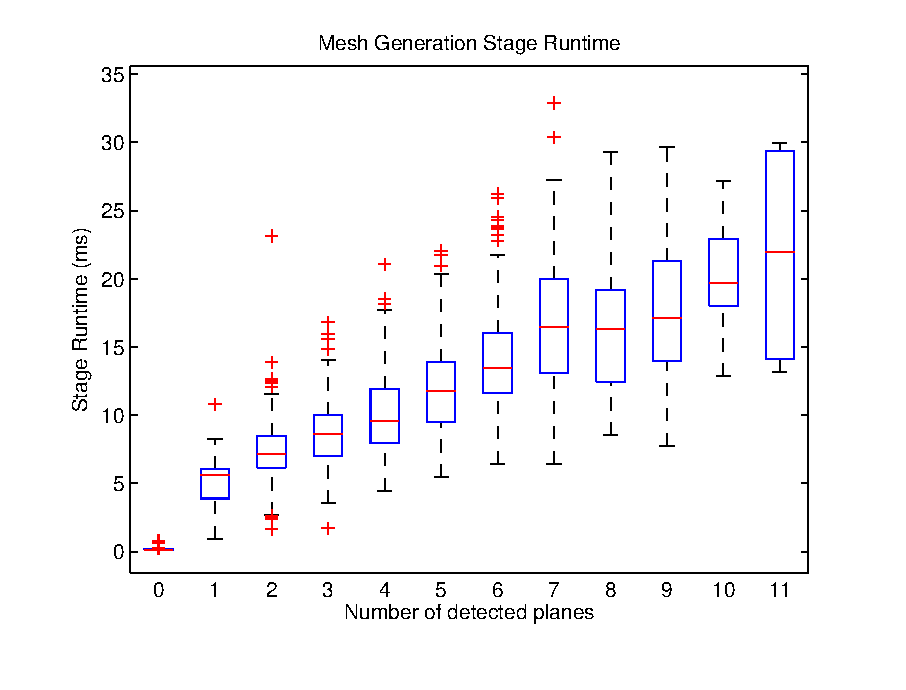
\includegraphics[width=0.7\textwidth]{MeshGenerationByNumPlanes.eps}
    \caption{Runtime of the mesh generation stage by number of detected planes.}
    \label{fig:meshgenerationplanes}
\end{figure}



\begin{figure}[ht]
    \centering
    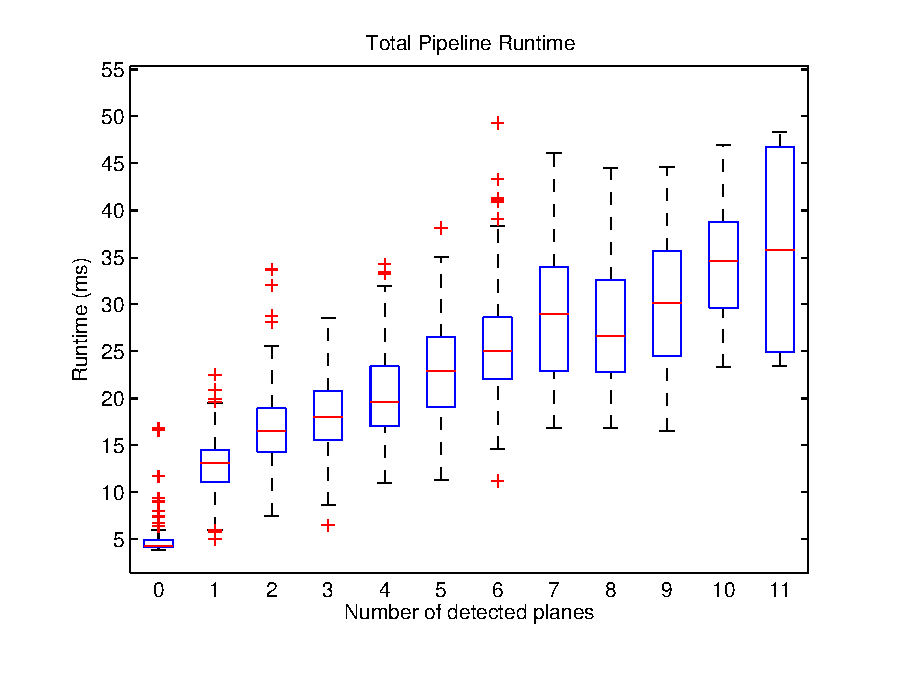
\includegraphics[width=0.7\textwidth]{PipelineByNumPlanes.eps}
    \caption{Runtime of the entire pipeline by number of detected planes.}
    \label{fig:pipelineplanes}
\end{figure}

